\documentclass{standalone}
\usepackage{tikz}
\usetikzlibrary{patterns, positioning}
\usepackage[sfdefault]{ClearSans} %% option 'sfdefault' activates Clear Sans as the default text font
\usepackage[T1]{fontenc}

\begin{document}
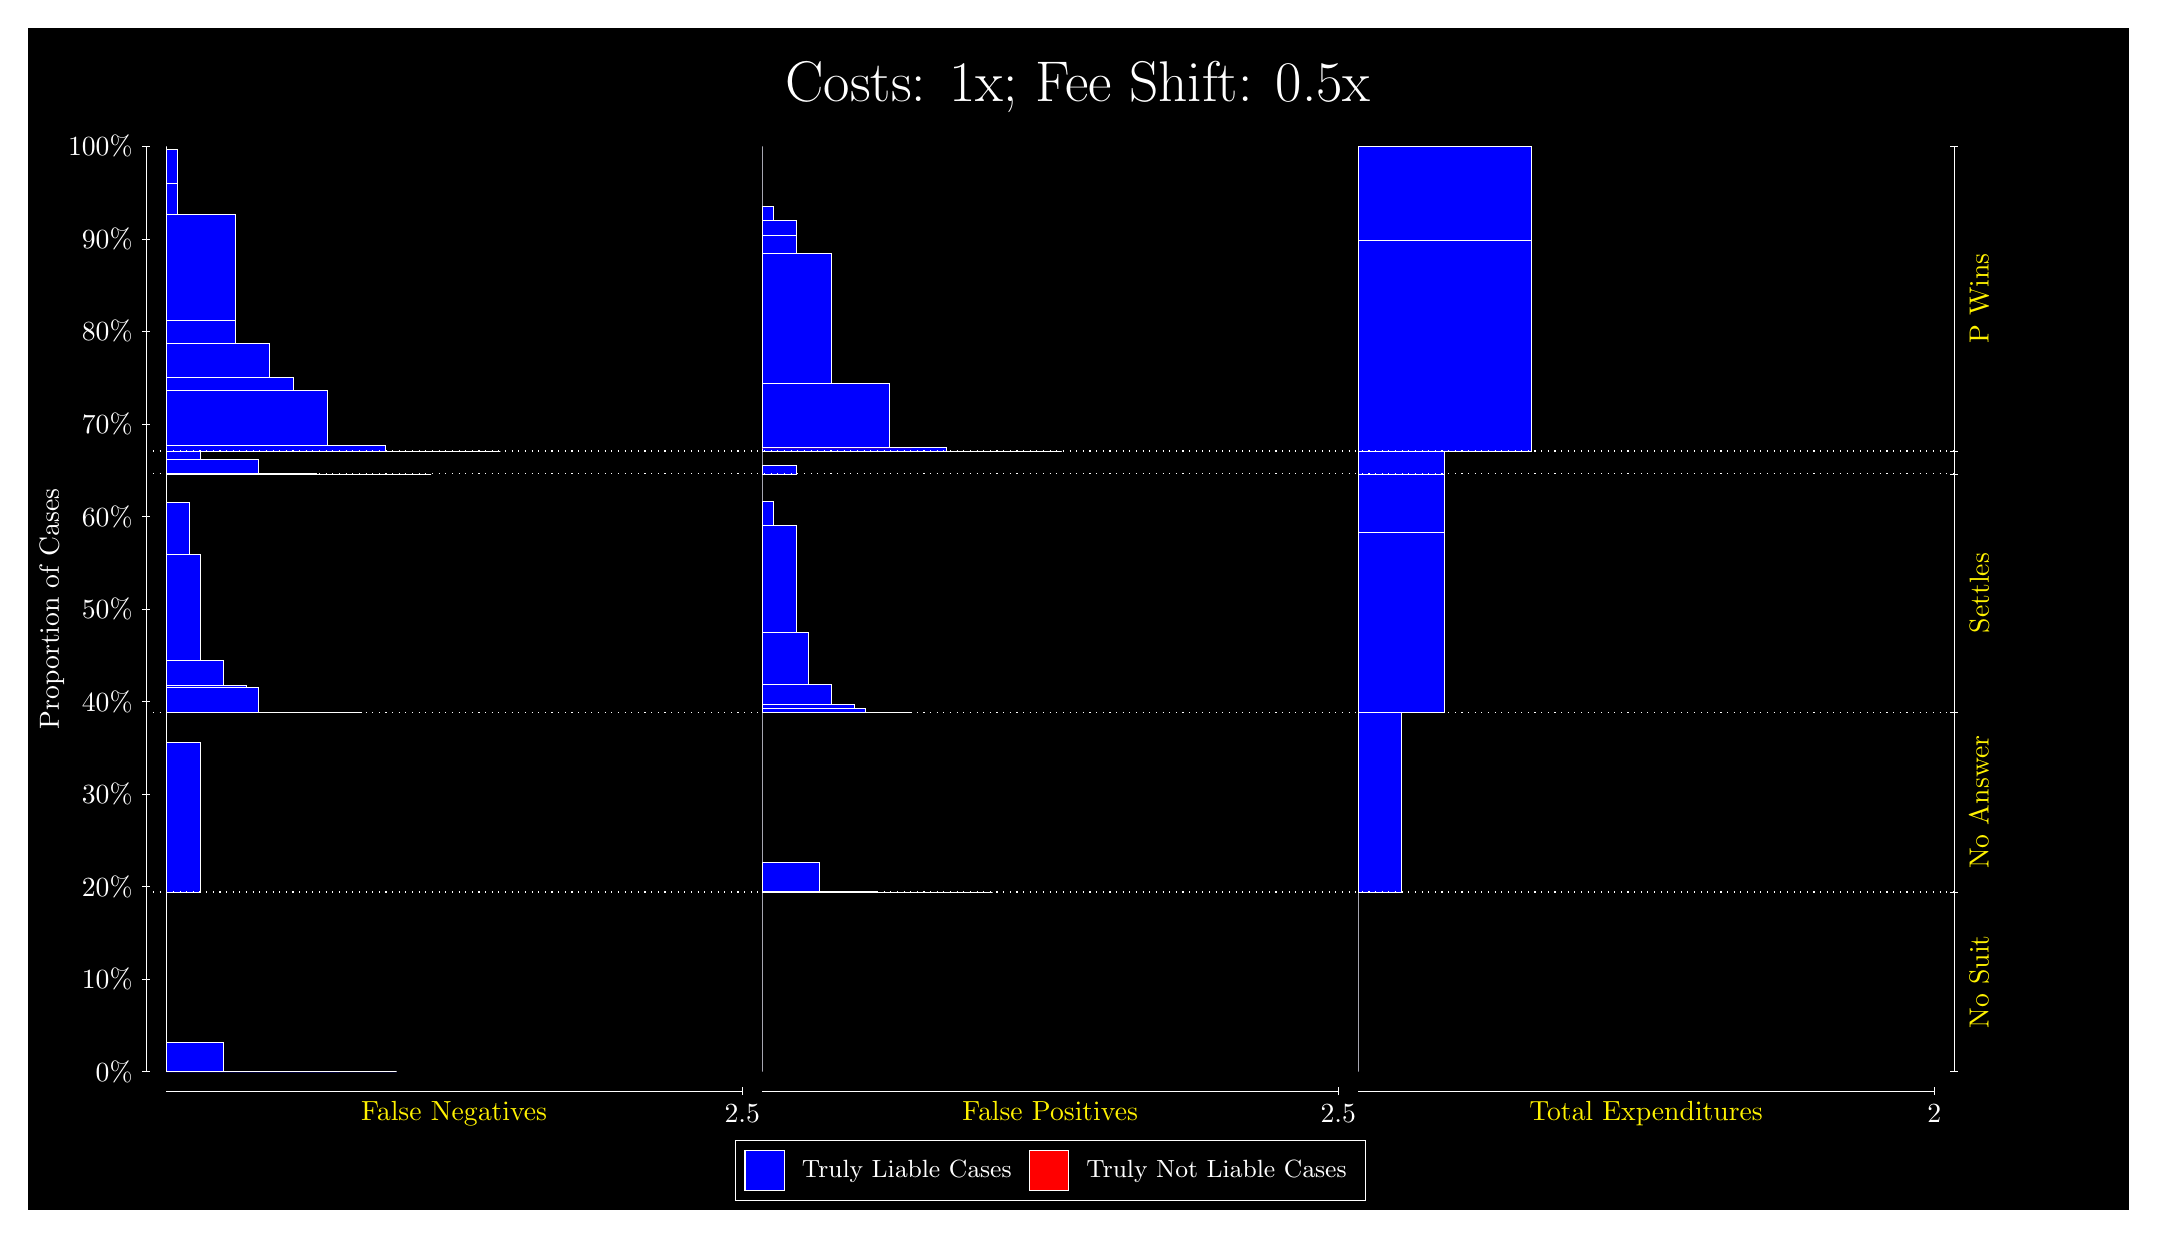
\begin{tikzpicture}
\draw[fill=black] (0,0) rectangle (26.667,15);
\draw[text=white] (0,13.5) rectangle (26.667,15) node[midway] {\huge Costs: 1x; Fee Shift: 0.5x};
\draw[white, very thin] (1.5,1.75) -- (1.5,13.5);
\node[rotate=90, text=white, anchor=center] at (0.3, 7.625) {Proportion of Cases};
\draw[white, very thin] (1.45,1.75) -- (1.55,1.75);
\node[text=white, anchor=east] at (1.45, 1.75) {0\%};
\draw[white, very thin] (1.45,2.925) -- (1.55,2.925);
\node[text=white, anchor=east] at (1.45, 2.925) {10\%};
\draw[white, very thin] (1.45,4.1) -- (1.55,4.1);
\node[text=white, anchor=east] at (1.45, 4.1) {20\%};
\draw[white, very thin] (1.45,5.275) -- (1.55,5.275);
\node[text=white, anchor=east] at (1.45, 5.275) {30\%};
\draw[white, very thin] (1.45,6.45) -- (1.55,6.45);
\node[text=white, anchor=east] at (1.45, 6.45) {40\%};
\draw[white, very thin] (1.45,7.625) -- (1.55,7.625);
\node[text=white, anchor=east] at (1.45, 7.625) {50\%};
\draw[white, very thin] (1.45,8.8) -- (1.55,8.8);
\node[text=white, anchor=east] at (1.45, 8.8) {60\%};
\draw[white, very thin] (1.45,9.975) -- (1.55,9.975);
\node[text=white, anchor=east] at (1.45, 9.975) {70\%};
\draw[white, very thin] (1.45,11.15) -- (1.55,11.15);
\node[text=white, anchor=east] at (1.45, 11.15) {80\%};
\draw[white, very thin] (1.45,12.325) -- (1.55,12.325);
\node[text=white, anchor=east] at (1.45, 12.325) {90\%};
\draw[white, very thin] (1.45,13.5) -- (1.55,13.5);
\node[text=white, anchor=east] at (1.45, 13.5) {100\%};

\draw[white, very thin] (24.457,1.75) -- (24.457,13.5);
\draw[white, very thin] (24.407,1.75) -- (24.507,1.75);
\node[anchor=west] at (24.407, 1.75) {};
\draw[white, very thin] (24.407,4.0302) -- (24.507,4.0302);
\node[anchor=west] at (24.407, 4.0302) {};
\draw[white, very thin] (24.407,6.3104) -- (24.507,6.3104);
\node[anchor=west] at (24.407, 6.3104) {};
\draw[white, very thin] (24.407,9.3412) -- (24.507,9.3412);
\node[anchor=west] at (24.407, 9.3412) {};
\draw[white, very thin] (24.407,9.6312) -- (24.507,9.6312);
\node[anchor=west] at (24.407, 9.6312) {};
\draw[white, very thin] (24.407,13.5) -- (24.507,13.5);
\node[anchor=west] at (24.407, 13.5) {};

\draw[white, very thin, fill=blue] (1.75,1.75) rectangle (4.6775,1.75);
\draw[white, very thin, fill=blue] (1.75,1.75) rectangle (3.9457,1.75);
\draw[white, very thin, fill=blue] (1.75,1.75) rectangle (3.2138,1.7532);
\draw[white, very thin, fill=blue] (1.75,1.7532) rectangle (2.4819,2.1234);
\draw[white, very thin, fill=red] (1.75,2.1234) rectangle (1.75,2.1234);
\draw[white, very thin, fill=blue] (1.75,2.1234) rectangle (1.75,4.0302);
\draw[white, very thin, fill=blue] (1.75,4.0302) rectangle (2.1891,5.937);
\draw[white, very thin, fill=red] (1.75,5.937) rectangle (1.75,5.937);
\draw[white, very thin, fill=blue] (1.75,5.937) rectangle (1.75,6.3104);
\draw[white, very thin, fill=blue] (1.75,6.3104) rectangle (4.2384,6.3104);
\draw[white, very thin, fill=blue] (1.75,6.3104) rectangle (3.9457,6.3104);
\draw[white, very thin, fill=blue] (1.75,6.3104) rectangle (3.6529,6.3111);
\draw[white, very thin, fill=blue] (1.75,6.3111) rectangle (3.5065,6.3111);
\draw[white, very thin, fill=blue] (1.75,6.3111) rectangle (3.2138,6.3137);
\draw[white, very thin, fill=blue] (1.75,6.3137) rectangle (2.921,6.6251);
\draw[white, very thin, fill=blue] (1.75,6.6251) rectangle (2.7746,6.66);
\draw[white, very thin, fill=blue] (1.75,6.66) rectangle (2.4819,6.9705);
\draw[white, very thin, fill=blue] (1.75,6.9705) rectangle (2.1891,8.3182);
\draw[white, very thin, fill=blue] (1.75,8.3182) rectangle (2.0428,8.9771);
\draw[white, very thin, fill=red] (1.75,8.9771) rectangle (1.75,8.9771);
\draw[white, very thin, fill=blue] (1.75,8.9771) rectangle (1.75,9.3412);
\draw[white, very thin, fill=blue] (1.75,9.3412) rectangle (5.1167,9.3412);
\draw[white, very thin, fill=blue] (1.75,9.3412) rectangle (4.3848,9.3412);
\draw[white, very thin, fill=blue] (1.75,9.3412) rectangle (3.6529,9.3474);
\draw[white, very thin, fill=blue] (1.75,9.3474) rectangle (2.921,9.529);
\draw[white, very thin, fill=blue] (1.75,9.529) rectangle (2.1891,9.6312);
\draw[white, very thin, fill=red] (1.75,9.6312) rectangle (1.75,9.6312);
\draw[white, very thin, fill=blue] (1.75,9.6312) rectangle (5.9949,9.6312);
\draw[white, very thin, fill=blue] (1.75,9.6312) rectangle (5.2631,9.6321);
\draw[white, very thin, fill=blue] (1.75,9.6321) rectangle (4.8239,9.6321);
\draw[white, very thin, fill=blue] (1.75,9.6321) rectangle (4.5312,9.6978);
\draw[white, very thin, fill=blue] (1.75,9.6978) rectangle (4.092,9.6978);
\draw[white, very thin, fill=blue] (1.75,9.6978) rectangle (3.7993,10.398);
\draw[white, very thin, fill=blue] (1.75,10.398) rectangle (3.3602,10.568);
\draw[white, very thin, fill=blue] (1.75,10.568) rectangle (3.0674,10.993);
\draw[white, very thin, fill=blue] (1.75,10.993) rectangle (2.6283,11.286);
\draw[white, very thin, fill=blue] (1.75,11.286) rectangle (2.6283,12.634);
\draw[white, very thin, fill=blue] (1.75,12.634) rectangle (2.3355,12.635);
\draw[white, very thin, fill=blue] (1.75,12.635) rectangle (1.8964,13.026);
\draw[white, very thin, fill=blue] (1.75,13.026) rectangle (1.8964,13.458);
\draw[white, very thin, fill=red] (1.75,13.458) rectangle (1.75,13.458);
\draw[white, very thin, fill=blue] (1.75,13.458) rectangle (1.75,13.5);
\draw[white, very thin, fill=red] (9.3189,1.75) rectangle (9.3189,1.75);
\draw[white, very thin, fill=blue] (9.3189,1.75) rectangle (9.3189,4.0302);
\draw[white, very thin, fill=red] (9.3189,4.0302) rectangle (12.246,4.0302);
\draw[white, very thin, fill=blue] (9.3189,4.0302) rectangle (12.246,4.0302);
\draw[white, very thin, fill=blue] (9.3189,4.0302) rectangle (11.515,4.0302);
\draw[white, very thin, fill=blue] (9.3189,4.0302) rectangle (10.783,4.0334);
\draw[white, very thin, fill=blue] (9.3189,4.0334) rectangle (10.051,4.4036);
\draw[white, very thin, fill=blue] (9.3189,4.4036) rectangle (9.3189,6.3104);
\draw[white, very thin, fill=red] (9.3189,6.3104) rectangle (11.222,6.3104);
\draw[white, very thin, fill=blue] (9.3189,6.3104) rectangle (11.222,6.3104);
\draw[white, very thin, fill=red] (9.3189,6.3104) rectangle (10.929,6.3104);
\draw[white, very thin, fill=blue] (9.3189,6.3104) rectangle (10.929,6.3111);
\draw[white, very thin, fill=red] (9.3189,6.3111) rectangle (10.636,6.3111);
\draw[white, very thin, fill=blue] (9.3189,6.3111) rectangle (10.636,6.3604);
\draw[white, very thin, fill=blue] (9.3189,6.3604) rectangle (10.49,6.4192);
\draw[white, very thin, fill=blue] (9.3189,6.4192) rectangle (10.197,6.6744);
\draw[white, very thin, fill=blue] (9.3189,6.6744) rectangle (9.9044,7.3334);
\draw[white, very thin, fill=blue] (9.3189,7.3334) rectangle (9.758,8.681);
\draw[white, very thin, fill=blue] (9.3189,8.681) rectangle (9.4652,8.9915);
\draw[white, very thin, fill=blue] (9.3189,8.9915) rectangle (9.3189,9.3412);
\draw[white, very thin, fill=red] (9.3189,9.3412) rectangle (9.758,9.3412);
\draw[white, very thin, fill=blue] (9.3189,9.3412) rectangle (9.758,9.4433);
\draw[white, very thin, fill=blue] (9.3189,9.4433) rectangle (9.3189,9.6312);
\draw[white, very thin, fill=red] (9.3189,9.6312) rectangle (13.125,9.6312);
\draw[white, very thin, fill=blue] (9.3189,9.6312) rectangle (13.125,9.6312);
\draw[white, very thin, fill=red] (9.3189,9.6312) rectangle (12.393,9.6312);
\draw[white, very thin, fill=blue] (9.3189,9.6312) rectangle (12.393,9.6317);
\draw[white, very thin, fill=red] (9.3189,9.6317) rectangle (11.661,9.6317);
\draw[white, very thin, fill=blue] (9.3189,9.6317) rectangle (11.661,9.6736);
\draw[white, very thin, fill=red] (9.3189,9.6736) rectangle (11.222,9.6736);
\draw[white, very thin, fill=blue] (9.3189,9.6736) rectangle (11.222,9.6736);
\draw[white, very thin, fill=red] (9.3189,9.6736) rectangle (10.929,9.6736);
\draw[white, very thin, fill=blue] (9.3189,9.6736) rectangle (10.929,10.497);
\draw[white, very thin, fill=red] (9.3189,10.497) rectangle (10.49,10.497);
\draw[white, very thin, fill=blue] (9.3189,10.497) rectangle (10.49,10.497);
\draw[white, very thin, fill=blue] (9.3189,10.497) rectangle (10.197,12.138);
\draw[white, very thin, fill=blue] (9.3189,12.138) rectangle (9.758,12.371);
\draw[white, very thin, fill=red] (9.3189,12.371) rectangle (9.758,12.371);
\draw[white, very thin, fill=blue] (9.3189,12.371) rectangle (9.758,12.564);
\draw[white, very thin, fill=blue] (9.3189,12.564) rectangle (9.4652,12.734);
\draw[white, very thin, fill=blue] (9.3189,12.734) rectangle (9.3189,13.5);
\draw[white, very thin, fill=red] (16.888,1.75) rectangle (16.888,1.75);
\draw[white, very thin, fill=blue] (16.888,1.75) rectangle (16.888,4.0302);
\draw[white, very thin, fill=red] (16.888,4.0302) rectangle (17.437,4.0302);
\draw[white, very thin, fill=blue] (16.888,4.0302) rectangle (17.437,6.3104);
\draw[white, very thin, fill=red] (16.888,6.3104) rectangle (17.986,6.3104);
\draw[white, very thin, fill=blue] (16.888,6.3104) rectangle (17.986,8.598);
\draw[white, very thin, fill=red] (16.888,8.598) rectangle (17.986,8.598);
\draw[white, very thin, fill=blue] (16.888,8.598) rectangle (17.986,9.3412);
\draw[white, very thin, fill=red] (16.888,9.3412) rectangle (17.986,9.3412);
\draw[white, very thin, fill=blue] (16.888,9.3412) rectangle (17.986,9.6312);
\draw[white, very thin, fill=red] (16.888,9.6312) rectangle (19.083,9.6312);
\draw[white, very thin, fill=blue] (16.888,9.6312) rectangle (19.083,12.308);
\draw[white, very thin, fill=red] (16.888,12.308) rectangle (19.083,12.308);
\draw[white, very thin, fill=blue] (16.888,12.308) rectangle (19.083,13.5);
\draw[white, dotted] (1.5,4.0302) -- (24.457,4.0302);
\draw[white, dotted] (1.5,6.3104) -- (24.457,6.3104);
\draw[white, dotted] (1.5,9.3412) -- (24.457,9.3412);
\draw[white, dotted] (1.5,9.6312) -- (24.457,9.6312);
\draw[white, very thin] (1.75,1.5) -- (9.0689,1.5);
\node[text=yellow, anchor=north] at (5.4094, 1.5) {False Negatives};
\draw[white, very thin] (9.0689,1.45) -- (9.0689,1.55);
\node[text=white, anchor=north] at (9.0689, 1.45) {2.5};

\draw[white, very thin] (9.3189,1.5) -- (16.638,1.5);
\node[text=yellow, anchor=north] at (12.978, 1.5) {False Positives};
\draw[white, very thin] (16.638,1.45) -- (16.638,1.55);
\node[text=white, anchor=north] at (16.638, 1.45) {2.5};

\draw[white, very thin] (16.888,1.5) -- (24.207,1.5);
\node[text=yellow, anchor=north] at (20.547, 1.5) {Total Expenditures};
\draw[white, very thin] (24.207,1.45) -- (24.207,1.55);
\node[text=white, anchor=north] at (24.207, 1.45) {2};

\node[text=yellow, centered, rotate=90] at (24.777, 2.8901) {No Suit};
\node[text=yellow, centered, rotate=90] at (24.777, 5.1703) {No Answer};
\node[text=yellow, centered, rotate=90] at (24.777, 7.8258) {Settles};

\node[text=yellow, centered, rotate=90] at (24.777, 11.566) {P Wins};

\draw (12.978300999999998,1.5) node[draw=none] (baseCoordinate) {};
\begin{scope}[align=center]
        \matrix[scale=0.5, draw=white, below=0.5cm of baseCoordinate, nodes={draw}, column sep=0.1cm]{
            \node[rectangle, draw, minimum width=0.5cm, minimum height=0.5cm, fill=blue] {}; &
            \node[draw=none, font=\small, text=white] (B) {Truly Liable Cases}; &
            \node[rectangle, draw, minimum width=0.5cm, minimum height=0.5cm, fill=red] {}; &
            \node[draw=none, font=\small, text=white] (B) {Truly Not Liable Cases}; \\
            };
\end{scope}

\end{tikzpicture}
\end{document}